\secnumbersection{DEFINICIÓN DEL PROBLEMA}

\subsection{Contexto}

En el mundo de la robótica existen diferentes categorías de competencias a lo largo del mundo. Una de las más antiguas es la All Japan Robotracer \& micromouse Contest\footnote{https://www.ntf.or.jp/, Página oficial de la competencia} con más de 40 años de trayectoria que consta de 2 categorías. Uno de los objetivos de esta competencia es ser un cuna para la innovación, diferentes empresas compiten acá para poner a pruebas nuevas tecnologías, y así evaluar su factibilidad y utilidad para luego poder implementarlas en aplicaciónes de la vida real. El enfoque de este trabajo va a ser en la categoría denominada Robotracer.

Las bases de la competencia de la categoría a trabajar son las siguientes: Se tiene una pista consistente de una linea blanca continua sobre fondo negro (Ver figura \ref{fig:pista1}). El robot debe ser capaz de recorrer la totalidad del trazado de forma válida, es decir, que la poryección del robot no se salda de este, y además detenerse por su cuenta. Esta pista no se conocida hasta el momento de participar, por lo que no se puede hacer un pre mapeado de la pista.

Se tienen 5 intentos dentro de un periodo de 3 minutos para lograr el menor tiempo posible. Lo normal es utilizar el primer intento para mapear la pista y los otros 4 para lograr vueltas válidas lo más rápido posible.

Aquí se puede ver la ronda del campeón actual de la competencia. \cite{ganador2023}

\begin{figure}[h]
\centering
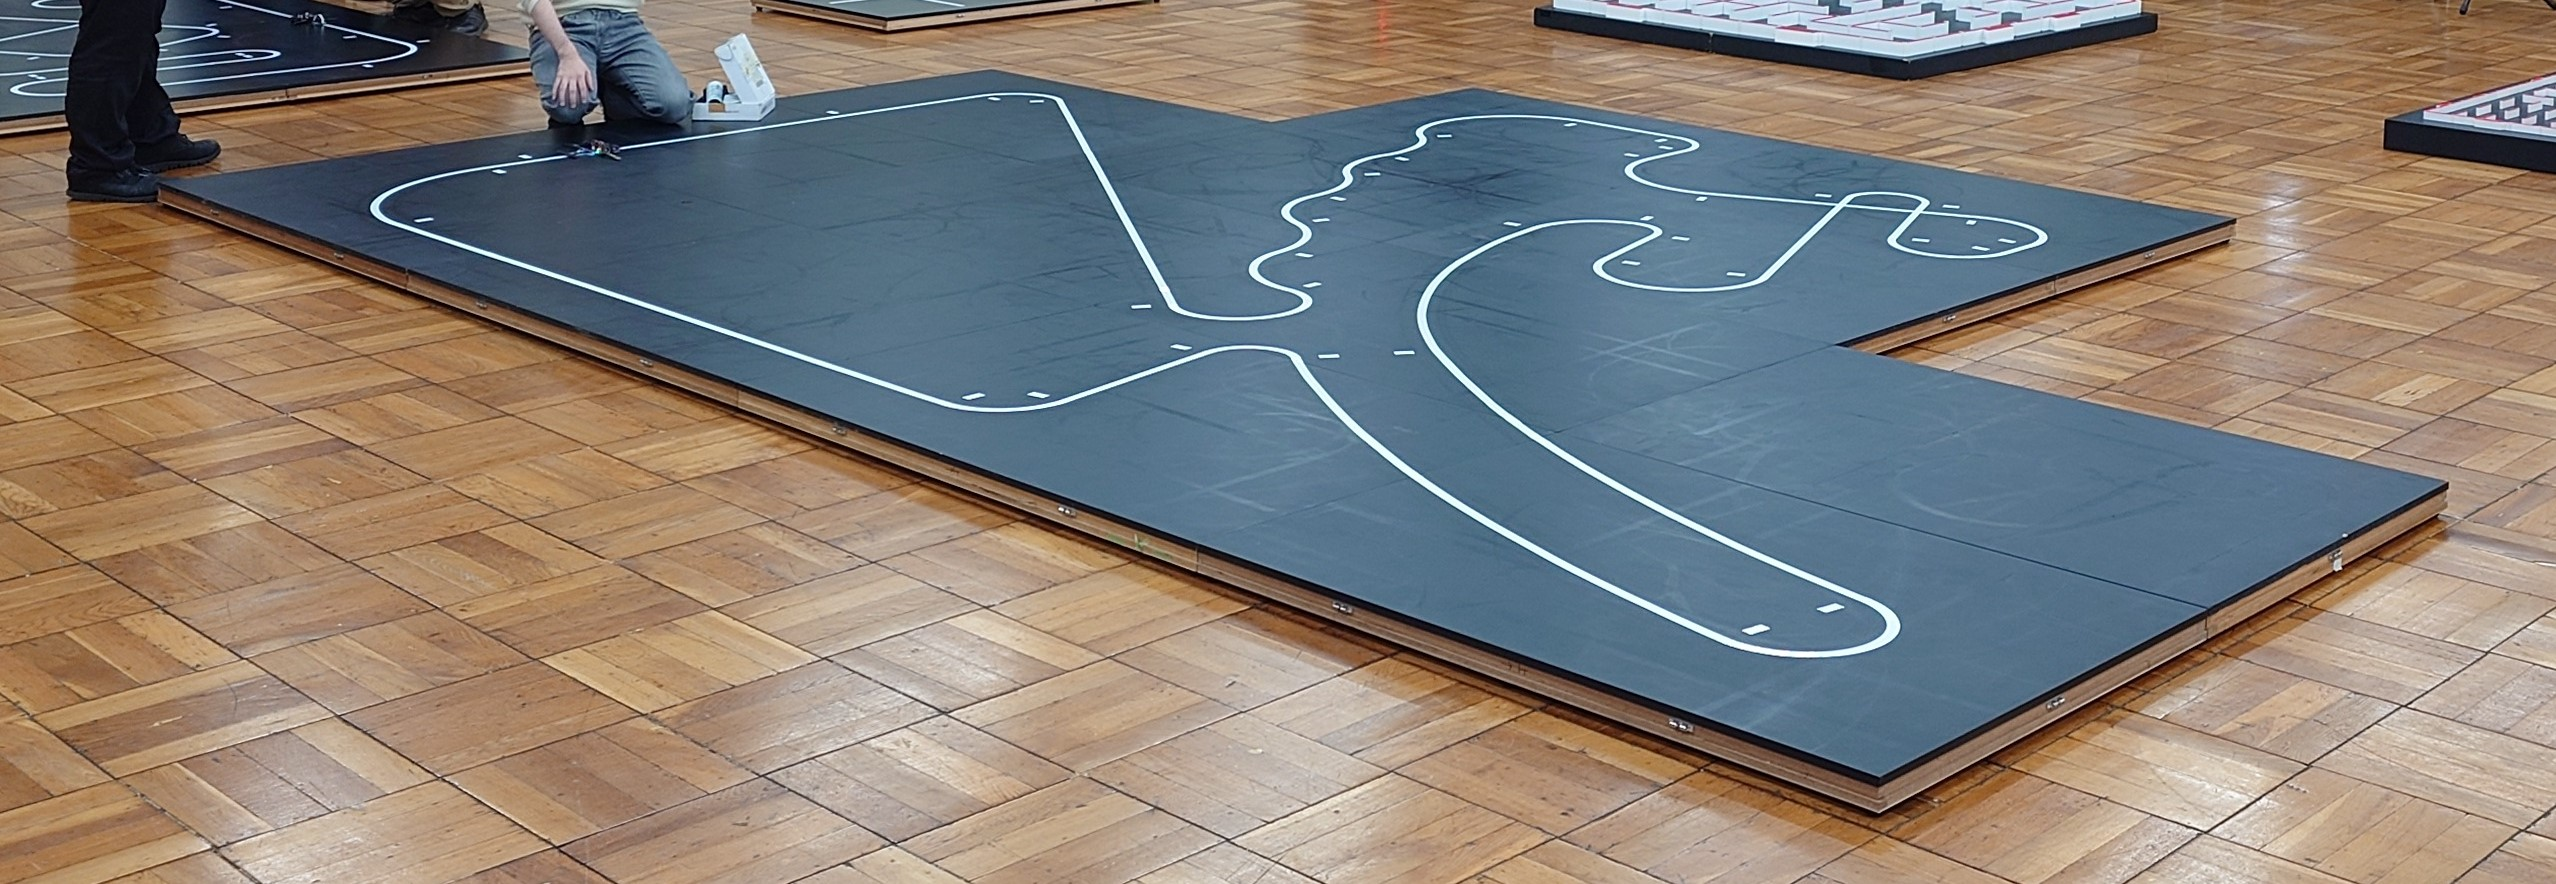
\includegraphics[width=0.8\textwidth]{ejemplo_pista_1}
\caption{\label{fig:pista1} Ejemplo de pista} Fuente: Elaboración propia.
\end{figure}

Los últimos años todos los esfuerzos de mejora se han enfocado en la mecánica y electrónica del robot, principalmente con la adición de métodos de succion mediante turbinas, dejando de lado el software. Es por este motivo que en la última versión no se ha otorgado el premio a la innovación a ningún participante.

\subsection{Arquitectura Actual}
En la última competencia realizada, la gran mayoría (por no decir todos), programaba sus robots en C/C++, aplicando algoritmos de MATLAB (más adelante se detalla). La ventaja de esto es que MATLAB genera scripts en C/C++, por lo que se pueden usar algoritmos de optimización preexistentes sin mayores complicaciones.



